%% Travail effectué
\section{BMC}

BMC, "Braille music compiler" est un programme qui se veut de transformer un fichier écris en "Braille Music" en un autre langage utilisable par d'autres applications. La difficulté est que le langage "Braille Music" possède beaucoup d'ambiguïtés, en effet par exemple pour connaitre la note exacte en cours, il est nécessaire de savoir quelles ont été les notes précédentes. A l'heure actuel le programme arrive correctement à compiler le langage "Braille Music" en un langage Abstrait qui lui ne possède aucune ambiguïté. Ce langage abstrait peut être converti en n'importe quels formats de musique. Par exemple : 
\begin{itemize}
\item MIDI
\item MusicXML
\item lilypond
\end{itemize}
\begin{figure}[!h]
  \centering
  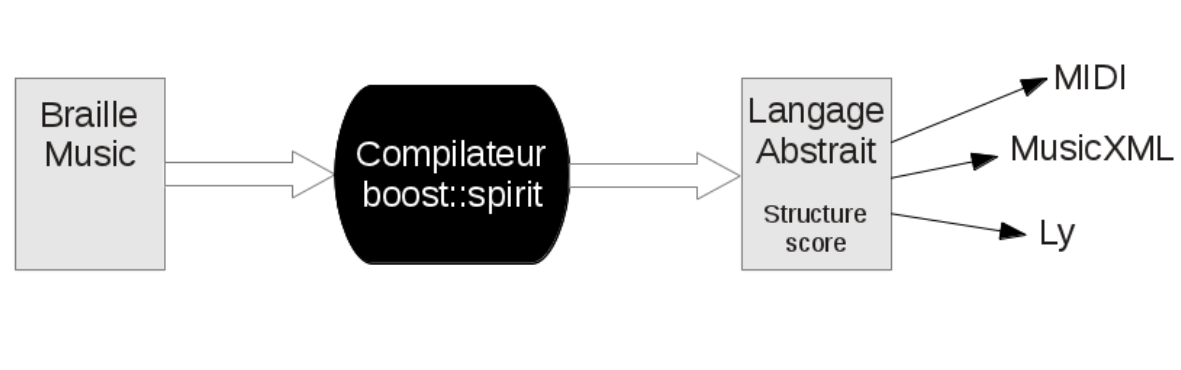
\includegraphics[scale=0.4]{images/fonction-bmc.png}
  \caption{Schéma visuel du fonctionement de BMC}
  
\end{figure}

Notre travail est donc d'implémenter ses modules de convesion. Pour cela il est nécessaire de comprendre comment est conçu le langage Abstrait. Après la compilation du "Braille Music", l'ensemble des données sont stockées dans une structure nommée "score". Cette structure est une multitude de vecteurs imbriqués les uns dans les autres. Voici le code de la strucure suivi d'une représentation visuel :

\begin{verbatim}
typedef boost::variant<note, rest, chord, value_distinction, hand_sign, simile, barline>;
typedef std::vector<sign> partial_voice;
typedef std::vector<partial_voice> partial_measure;
typedef std::vector<partial_measure> voice;
struct measure : locatable
{
  boost::optional<unsigned> ending;
  std::vector<voice> voices;
};
typedef std::vector< boost::variant<measure> > staff;
typedef std::vector<staff> part;
struct score {
  boost::optional<time_signature> time_sig;
  std::vector<part> parts;
};
\end{verbatim}

\begin{figure}[!h]
  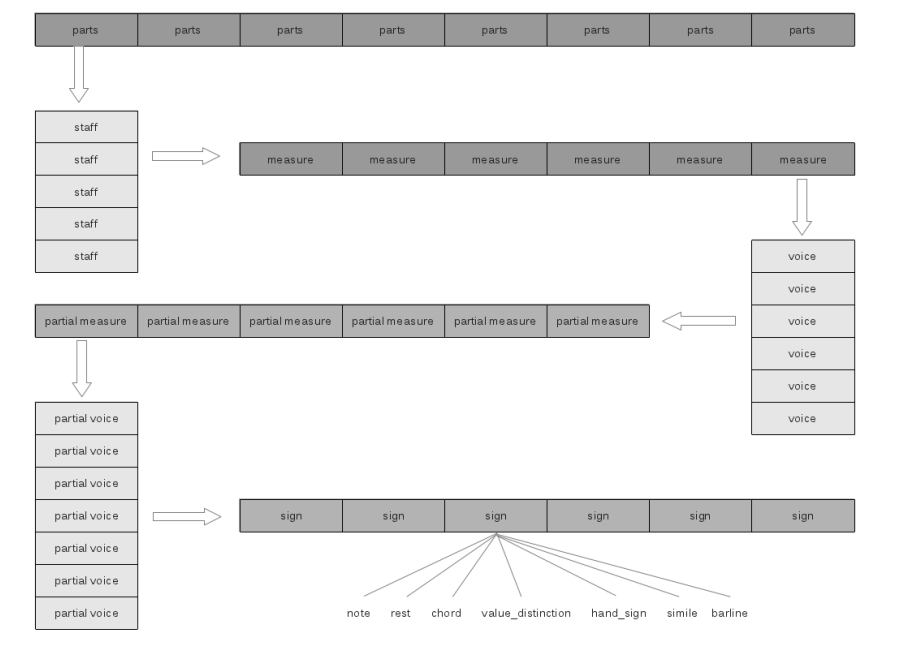
\includegraphics[scale=0.8]{images/bmc-score.png}
  \caption{Représentation de la structure score}
\end{figure}

Il est donc maintenant plus facile d'expliquer la structure score. Un fichier de musique braille peut donc se diviser en plusieurs partie (parts). Chaque partie possède un ou plusieurs "staff". Un "staff" n'est autre que la portée, typiquement si le compositeur écris une partition de musique pour piano il y aura deux portées. Chaque portée possède un nombre de mesures. Si la musique composée est polyphonique il y aura plusieurs voix ("voices"). Une voix est ensuite divisée en mesures partielles ... ( // TODO )).


\begin{figure}[!h]
  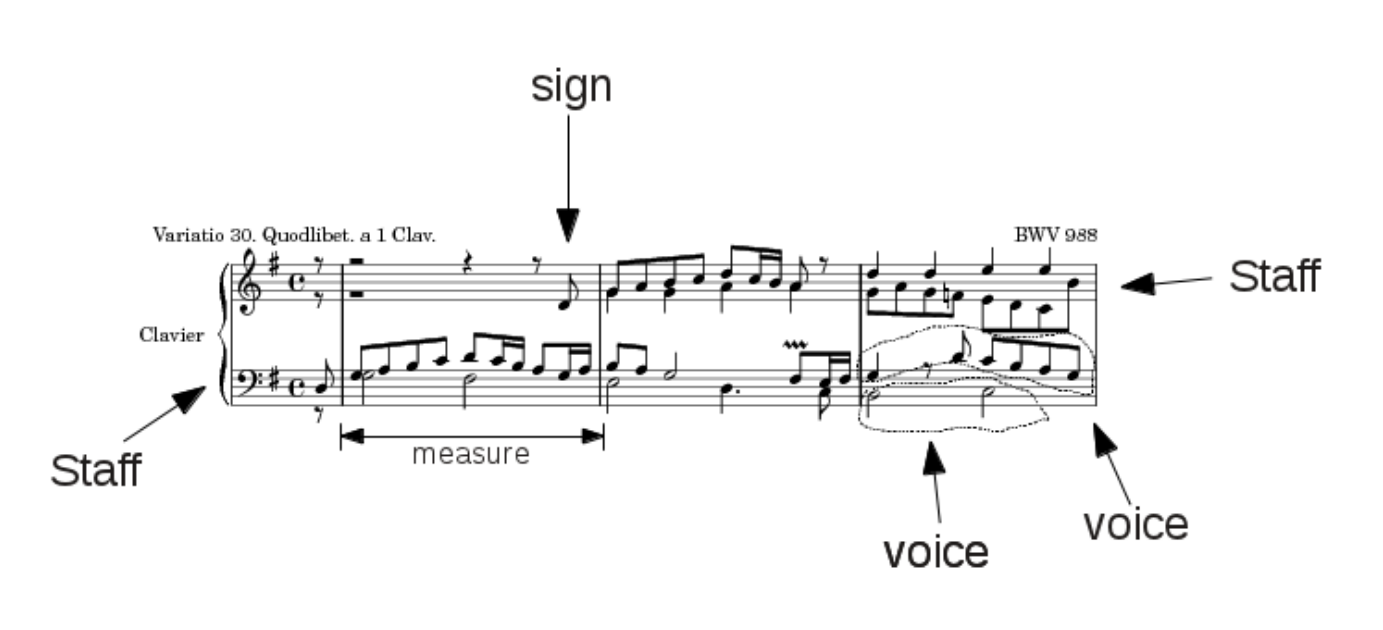
\includegraphics[scale=0.4]{images/score-visu.png}
  \caption{Un petit exemple visuel}
\end{figure}

Avant de se mettre à faire la conversion du langage abstrait vers un format de musique conventionel nous avons d'abord créer les classes de bases que nous devrons utilisées pour effectuer les différentes conversions. On procède à un affichage sur le terminal dans un premier temps.

\begin{verbatim}
./bmc < input/bwv988-v30.bmc 

 r1/8  r1/8 >  |   r1/2  r1/4  r1/8 D 5 >   r1/1 >  |  G 5 A 5 B 5 C 6 D 
6 C 6 B 5 A 5  r1/8 >  G 5 G 5 A 5 A 5 >  |  D 6 D 6 E 6 E 6 >  G 5 A 5 G 
5 F 5 Natural  E 5 D 5 C 5 B 5 >  |  B 5 A 5 G 5 G 5 G 5 D 5 >  |   r1/2 
 r1/4  r1/8 D 6 >  G 5 A 5 B 5 C 6 D 6 C 6 B 5 A 5 D 6 >  G 5 G 5 A 5 A 5 > 
\end{verbatim}

\section{Interface graphique}

L'un des critères essentiels de ce projet est l'accessibilité. Par
conséquent, nous avons choisi d'utiliser la bibliothèque GTK+ pour
l'interface graphique sur plateforme linux. En effet, cette
bibliothèque est compatible avec les lecteurs d'écran des systèmes
linux.


\subsection*{Forme}
L'interface graphique est très classique: elle présente une barre de
menu, une barre de raccourcis ainsi que les raccourcis naturels,
encore en cours d'implémentation. La fenêtre se divise en deux
parties: la premiere partie sert pour l'utilisateur malvoyant à éditer les partitions braille. La
deuxième partie sert à l'utilisateur voyant à avoir une partition
classique.

\begin{center}
\begin{figure}[!h]
  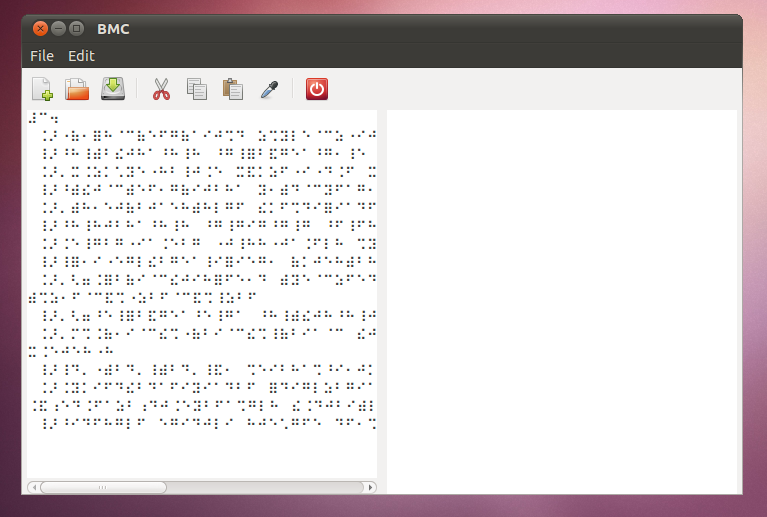
\includegraphics[scale=0.65]{images/linux_gui.png}
  \caption{Représentation de la structure score}
\end{figure}
\end{center}



\subsection*{Fonctionnalitées}
Le prototype réalisé comporte tous les fonctionnalitées de base d'un
éditeur de texte. Il permet de créer un nouveau fichier, d'ouvrir un
fichier, d'enregistrer un fichier et d'enregistrer le fichier courant
sous un autre nom. Il permet aussi d'éditer les textes avec les outils
classiques comme copier, couper, coller, séléctionner du texte.
\\ Non seulement, toutes ces fonctions sont accèssible depuis la barre
de menu et/ou la barre d'outils, elles sont également toutes associées
avec des raccourci clavier. Les raccourci utilisés sont très
classiques. Par exemple, Ctrl + o pour ouvrir, Ctrl + c pour copier et
Ctrl + v pour coller.
\\ Le prototype possède aussi une procedure de
sécurité qui consiste à vérifier si le fichier en cours d'édition est
sauvegardé ou non et propose à l'utilisateur d'enregistrer son
fichier lorsque l'utilisateur tente de créer un nouveau fichier,
d'ouvrir un autre fichier ou encore de quitter le programme.




\section{Bibliotèque BOOST}

Lors de notre analyse du langage abstrait et ce en scrutant de plus près le code source du \textit{Braille Music Compiler} nous étions amenés à étudier la bibliothèque BOOST  qui est un ensemble de bibliothèques C++ gratuites et portables. BOOST est très riche et fournit un large choix de bibliothèques, mais nous ne préciserons que celles utilisées pour le stockage de la music sous forme de langage abstrait.


\subsection*{Boost.Variant}

Le Boost.Variant est une sorte de type \textit{somme}. Il s'agit en fait de décomposer un type donné en plusieurs sous-types. Une instance de ce type donné peut être obtenue par une valeur de ses sous-types, mais pas deux types à la fois. Ce qui peut être assimiler à une \textit{union}. Cependant, en \textit{C} et \textit{C++} le type \textit{union} ne permet pas de gérer des classes dès qu'elles ont un constructeur ce qui est rendu possible grâce au Boost.Variant en \textit{C++}.

Donc contrairement à un \textit{std::vector} en C++ qui offre des éléments \textit{multi-valeur, type unique}, le \textit{boost::variant} quant à lui offre des éléments \textit{multi-type, valeur unique}.

%Dans le cadre de notre projet, le boost variant nous permet de

\subsection*{Boost.rational}

Le langage C++ offre plusieurs possibilités de stocker des nombres, des entiers naturels au réels et ce en les approximants pa différents types : unsigned int, int, float... La bibliothèque boost.rational permet de représenter un nouveau groupe de nombre : Les nombres rationnels.

Au niveau implémentation le type Boost.rational est constitué de deux nombres type entier, qui représente le numérateur et le dénominateur. De cette façon, cela permet d'avoir une meilleure précision de calcul et faciliter l'implémentation.


